\section{Implementacja}

Implementacja właściwa filtrowania metodą Savitzky-Golay została przygotowana z wykorzystaniem języka C++ w standardzie C++11. Filtracja z uwagi na niewielkie wykorzystanie zasobów wykonywana jest w głównym wątku programu. 
Aplkacja pobiera z linii poleceń wszystkie niezbędne parametry takie jak nazwy plików wejściowego i wyjściowego, szerokość okna filtracji, rząd wykorzystanego wielomianu oraz parametr decydujący czy po zakończeniu obliczeń pokazać wykres porównujący sygnał surowy i przefiltrowany. Procedura zbudowania i uruchomienia aplikacji opisana jest w Dodatku \ref{sec:how_to}.



\subsection{Wykorzystane biblioteki}
W aplikacji wykorzystano bilbiotekę Eigen (http://eigen.tuxfamily.org), która dostarcza funkcjonalności umożliwiające operować na wektorach i macierzach w sposób znany nam chociażby ze środowiska Matlab. Biblioteka oparta jest o szablony. Nie wymaga ona instalacji, gdyż dystrybuowana jest jako zbiór plików nagłówkowych, które wystarczy (opcjonalnie wybiórczo) umieścić w swoim projekcie.

Biblioteka Eigen oferuje użytkownikom typy o dynamicznie ustalanym rozmiarze reprezentujące wektor i macierz (np. liczb typu float):
\begin{itemize}
  \item Eigen::VectorXf
  \item Eigen::MatrixXf
\end{itemize}

Dodatkowo dostarcza przydatne funkcje jak:
\begin{itemize}
  \item Eigen::MatrixXf transpose() - zwracającą transpozycję macierzy,
  \item Eigen::MatrixXf inverse() - zwracającą macierz odwrotną.
\end{itemize}


\subsection{Wyjście programu}
Wyjściem programu jest plik z danymi. Plik posiada następujący format:
\begin{center}
\begin{lstlisting}[frame=single]
Time[s] MLII[mV] MLII_Filtered[mV] V5[mV] V5_Filterred[mV]
     0   -0.145 -0.314107         -0.065 -0.216375
 0.003   -0.145 -0.314043         -0.065 -0.216346
 0.006   -0.145 -0.313977         -0.065 -0.216311
 0.008   -0.145 -0.313882         -0.065 -0.216267
 0.011   -0.145 -0.313774         -0.065 -0.21621
 0.014   -0.145 -0.313648         -0.065 -0.216148
 0.017   -0.145 -0.313519         -0.065 -0.216095
 0.019   -0.145 -0.313392         -0.065 -0.216052
 0.022   -0.12  -0.313274         -0.08  -0.216001
\end{lstlisting}
\end{center}

Opcjonalnie na podstawie takiego pliku można wygenerować wykres z porównaniem sygnału przed i po filtracją. Wykres generowany jest przez środowisko \textbf{gnuplot}. Przykładowy wykres przedstawiono poniżej.

\begin{figure}[H]
  \begin{center}
    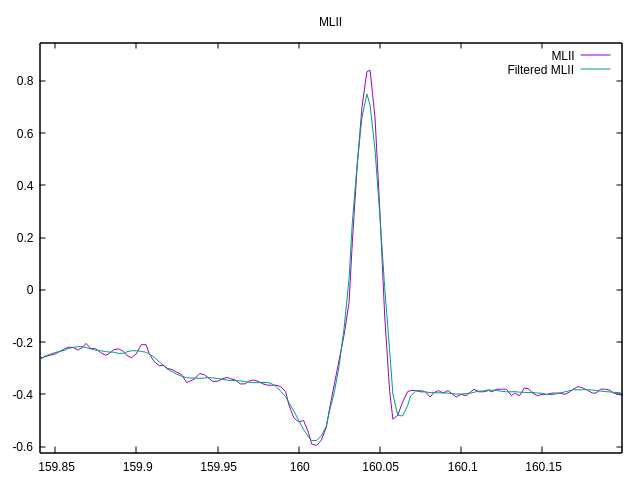
\includegraphics[scale=0.8]
    {img/implem.png}
  \end{center}
  \caption{Porównanie sygnałów przy filtracji wielomianem $N=2$ stopnia serii $2M+1=15$ próbek}
  \label{rys:implem}
\end{figure}


\subsection{Porównanie z modelem programowym}

Poniżej przedstawiono porównanie sygnałów przefiltrowanych w prototypie oraz we właściwej aplikacji. Nie widać większych różnic między sygnałami.


\begin{figure}[H]
  \begin{center}
    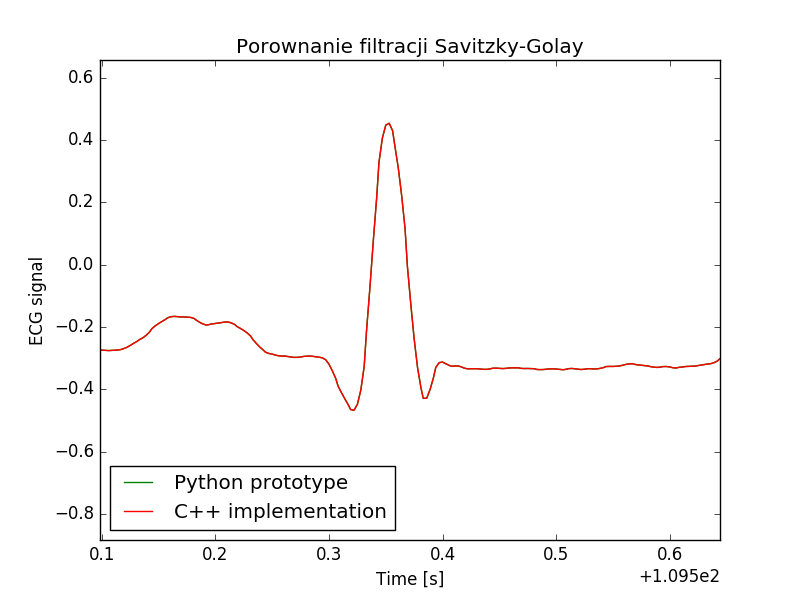
\includegraphics[scale=0.8]
    {img/implem_vs_proto.png}
  \end{center}
  \caption{Rozbieżności przy filtracji wielomianem $N=2$ stopnia serii $2M+1=21$ próbek}
  \label{rys:implem1}
\end{figure}


Aby upewnić się jaka rozbieżność istnieje między sygnałami policzono błąd średniokwadratowy, jako odniesienie przyjmując wynik filtracji z użyciem funkcji \texttt{scipy.signal.savgol\_filter()}. Wzięto pod uwagę 100 000 próbek, czyli 277 sekund sygnału EKG. 
\begin{equation}
MSE = \dfrac{1}{n} \sum\limits_{i=0}^n (x_i - \hat{x_i})^2 
\end{equation}
gdzie $x$ to sygnał badany, $\hat{x}$ to sygnał wzorcowy, a $n$ to długość sygnałów.

Wyniki zebrano w tabeli \ref{tab:mse}.

\begin{table}[!htb]
  \centering
  \begin{tabular}{|c|c|c|c|}
  \hline 
  Sygnał badany  & MSE \\  
  \hline 
  MIT-BIH 100, filtracja: prototyp & 2.75e-29 \\
  \hline
  MIT-BIH 100, filtracja: C++ & 1.96e-9 \\
  \hline
\end{tabular} 
\caption{Parametry filtru}
\label{tab:mse}
\end{table}

Warto zauważyć, że sygnały z bazy MIT-BIH charakteryzują się rozdzielczością kwantyzacji $5 \cdot 10^{-6} V$, ponieważ wersja cyfrowa była tworzona przy użyciu przetwornika 11-bitowego w zakresie $10 mV$. Jak widać, metody na większości sygnału działają identycznie. Różnica pojawia się dla ostatnich $M$ próbek, ze względu na drobne różnice w traktowaniu wartości brzegowych.